\documentclass[12pt]{article}
\usepackage{JASA_manu} %formats document like ASA wants
\usepackage{natbib} %formats citations like ASA wants
\usepackage{amssymb, amsmath, amsthm, graphics, graphicx, color, fullpage}
\usepackage{psfrag,epsf}
\usepackage{enumerate}
\usepackage{thmtools} %to format the Algorithm environment correctly
%\usepackage{hyperref}
%\hypersetup{
%  colorlinks   = true,    % Colours links instead of ugly boxes
%  urlcolor     = blue,    % Colour for external hyperlinks
%  linkcolor    = blue,    % Colour of internal links
%  citecolor    = red      % Colour of citations
%}
\usepackage{nameref, cleveref} %for named references
\usepackage[page,header]{appendix}
\usepackage{titletoc}
\usepackage{subcaption} % for subfigures

% define algorithm environment
\declaretheoremstyle[
notefont=\bfseries, notebraces={}{},
bodyfont=\normalfont\itshape,
headformat=\NAME:\NOTE
]{nopar}
\declaretheorem[style=nopar, name=Algorithm,
refname={Algorithm,Algorithms},
Refname={Algorithm,Algoritms},
numbered=no]{alg*}

\newtheorem{lem}{Lemma}

\DeclareMathOperator{\tr}{tr}
\DeclareMathOperator{\B}{B}
\DeclareMathOperator{\vech}{vech}
\DeclareMathOperator{\vect}{vec}

\graphicspath{{plots/}}

%\newcommand{\blind}{0}
%uncomment for compiling separately


\begin{document}

\def\spacingset#1{\renewcommand{\baselinestretch}%
{#1}\small\normalsize} \spacingset{1}
\setlength{\tabcolsep}{2pt}

\if0\blind
{
  \title{\bf Interweaving Markov Chain Monte Carlo Strategies for Efficient
    Estimation of Dynamic Linear Models}
  \author{Matthew Simpson\thanks{
    The authors thank the participants of the Economics, Finance, and Business workshop at the Bayes 250 conference and of the 2014 Bayesian Young Statisticians meeting for helpful comments, though all errors are our own.}\hspace{.2cm}\\
    Departments of Statistics and Economics, Iowa State University\\~\\
    Jarad Niemi \\
    Department of Statistics, Iowa State University\\~\\
    Vivekananda Roy\\
    Department of Statistics, Iowa State University}
  \maketitle
} \fi

\if1\blind
{
  \bigskip
  \bigskip
  \bigskip
  \begin{center}
    {\LARGE\bf Interweaving Markov Chain Monte Carlo Strategies for Efficient
    Estimation of Dynamic Linear Models}
\end{center}
  \medskip
} \fi

\bigskip


\begin{abstract}
In dynamic linear models (DLMs) with unknown fixed parameters, a standard Markov chain Monte Carlo (MCMC) sampling strategy is to alternate sampling of latent states conditional on fixed parameters and sampling of fixed parameters conditional on latent states. In some regions of the parameter space, this standard data augmentation (DA) algorithm can be inefficient. To improve efficiency, we seek to employ the interweaving strategies of \citet{yu2011center} that combine separate DAs by weaving them together. For this, we introduce a number of novel alternative DAs for a general class of DLMs: the scaled errors, wrongly-scaled errors, and wrongly-scaled disturbances. With the latent states and the less commonly used scaled disturbances, this yields five unique DAs to employ in MCMC algorithms. Each DA implies a unique MCMC sampling strategy and they can be combined into interweaving or alternating strategies that improve MCMC efficiency. We assess the strategies using the local level DLM and demonstrate that several strategies improve efficiency relative to the standard approach, the most efficient being either interweaving or alternating the scaled errors and scaled disturbances. Supplementary materials are available for this article online.
\end{abstract}


\noindent%
{\bf Key Words:} Ancillary augmentation; Centered parameterization; Data augmentation; Non-centered parameterization; Reparameterization; Sufficient augmentation; Time series; State-space model

\spacingset{2}

\section{Introduction}

The Data Augmentation (DA) algorithm of \citet{tanner1987calculation} and the closely related Expectation Maximization (EM) algorithm of \citet{dempster1977maximum} have become widely used strategies for computing posterior distributions and maximum likelihood estimates, with a long history of using ideas from the EM literature to inform the construction of DA algorithms and vice versa \citep{meng1997algorithm,van2010cross}. While useful, DA and EM algorithms often suffer from slow convergence s a large literature has grown up around various possible improvements to both algorithms \citep{meng1997algorithm,meng1999seeking,liu1999parameter,hobert2008theoretical,yu2011center}, though much of the work on constructing improved algorithms has focused on hierarchical models \citep{gelfand1995efficient,roberts1997updating,meng1998fast,van2001art,bernardo2003non,papaspiliopoulos2007general,papaspiliopoulos2008stability}. Despite some similarities with some hierarchical models, relatively little attention has been paid to time series models. Exceptions include \citep{pitt1999analytic,fruhwirth2003bayesian,fruhwirth2006auxiliary} in the DA literature and\citep{van2003one} in the EM literature. 

We seek to improve DA schemes in dynamic linear models (DLMs), i.e. linear Gaussian state-space models. The standard DA scheme uses the latent states and alternates between drawing from the full conditional distributions of the latent states and the model parameters \citep{fruhwirth1994data,carter1994gibbs}. The existing literature on improving DA algorithms in time series models tends to focus on non-Gaussian state-space models --- particularly the stochastic volatility model and models based on it \citep{shephard1996statistical,fruhwirth2003bayesian,roberts2004bayesian,bos2006inference,strickland2008parameterisation,fruhwirth2008heston,kastner2013ancillarity}, but a few work with the class of DLMs we consider \citep{fruhwirth2004efficient}. One recent development in the DA literature is an ``interweaving'' strategy for using two separate DAs in a single algorithm \citep{yu2011center}. This strategy draws on the strengths of both underlying DA algorithms in order to construct an MCMC algorithm which is at least as efficient as the worst of the two DA algorithms and typically at least as efficient as the best. We implement interweaving algorithms in a general class of DLMs and in order to do so we introduce several new DAs for this class of models. We also show under some assumptions that no {\it practical} sufficient augmentation (centered augmentation) exists for the DLM, which restricts the sort of interweaving algorithms we can construct. Using the local level model, we fit the model to simulated data using a variety of the MCMC strategies we discuss in order to assess their relative performance.

The rest of the paper is organized as follows. In Section \ref{sec:DA} we review the DA literature while in Section \ref{sec:DLM} we introduce the dynamic linear model and discuss the subclass of DLMs we consider. Section \ref{sec:DAs} explores several possible DAs for our class of DLMs and shows that any sufficient augmentation is likely to be difficult to use. Section \ref{sec:Algs} discusses the various MCMC strategies available for the DLM while Section \ref{sec:LLM} applies these algorithms to the local level model. Finally, Section \ref{sec:Discuss} discusses these results and suggests directions for further research while Section \ref{sec:Supp} contains an index to the supplementary materials.

\section{Variations of data augmentation}\label{sec:DA}

Suppose $p(\phi|y)$ is a probability density, for example the posterior distribution of some parameter $\phi$ given data $y$. %We use $p(.)$ to denote the probability density of the enclosed random variables.
Then a DA algorithm adds a DA $\theta$ with joint distribution $p(\phi,\theta|y)$ such that $\int_{\Theta}p(\phi,\theta|y)d\theta = p(\phi|y)$. The DA algorithm is a Gibbs sampler for $(\phi,\theta)$, except we focus attention on the marginal chain for $\phi$. In this DA algorithm, the $k+1$'st state of $\phi$ is obtained from the $k$'th state as follows (we implicitly condition on the data $y$ in all algorithms and only superscript the previous and new draws of the model parameters of interest):
\begin{alg*}[DA]Data Augmentation\label{alg:DA}
{\small
\begin{center}
  \begin{tabular}{lll}
  $[\theta|\phi^{(k)}]$ &$\to$& $[\phi^{(k+1)}|\theta]$
\end{tabular}
\end{center}
}
\end{alg*}
\noindent where $[\theta|\phi^{(k)}]$ means a draw of $\theta$ from $p(\theta|\phi^{(k)},y)$ and $[\phi^{(k+1)}|\theta]$ means a draw from $p(\phi|\theta,y)$. The DA need not be interesting in any scientific sense --- it can be viewed purely as a computational construct. 

\subsection{Reparameterization and alternating DAs}

One well known method of improving mixing and convergence in MCMC samplers as well as convergence in EM algorithms is reparameterization of the model (see  \citet{papaspiliopoulos2007general} and references therein). The DA $\theta$ is called a {\it sufficient augmentation} (SA) for the model parameter $\phi$ if $p(y|\theta,\phi)=p(y|\theta)$. Similarly $\theta$ is called an {\it ancillary augmentation} (AA) for $\phi$ if $p(\theta|\phi)=p(\theta)$. An SA is sometimes called a centered augmentation or centered parameterization in the literature while an AA is sometimes called a non-centered augmentation or non-centered parameterization. Like \citet{yu2011center} we prefer the SA and AA terminology because it suggests a connection with Basu's theorem \citep{basu1955statistics}, which we will return to in Section \ref{sec:Intro:int}.

A key reason behind the emphasis on SAs and AAs is that typically when the DA algorithm based on the SA has nice mixing and convergence properties, the DA algorithm based on the AA has poor mixing and convergence properties and vice-versa. This property suggests combining the two such DA algorithms to construct an improved sampler. One intuitive approach is to alternate between the two augmentations within a Gibbs sampler \citep{papaspiliopoulos2007general}. Suppose we have a second distinct DA $\gamma$ such that $\int_\Gamma p(\phi,\gamma|y)d\gamma = p(\phi|y)$, then the alternating algorithm for sampling from $p(\phi|y)$ is as follows:
\begin{alg*}[Alt]Alternating Algorithm\label{alg:Alt}
{\small
  \begin{center}
    \begin{tabular}{lllllll}
  $[\theta|\phi^{(k)}]$& $\to$& $[\phi|\theta]$& $\to$& $[\gamma|\phi]$& $\to$& $[\phi^{(k+1)}|\gamma]$.
    \end{tabular}
  \end{center}
}
\end{alg*}
\noindent One iteration of the alternating algorithm consists of one iteration of the DA algorithm based on $\theta$ to obtain an intermediate value of $\phi$, followed by one iteration of the DA algorithm based on $\gamma$.

When $\phi$ and $\theta$ are highly dependent in their joint posterior, the draws from $p(\theta|\phi,y)$ and $p(\phi|\theta,y)$ will hardly move the chain in Algorithm \nameref{alg:DA}, resulting in high autocorrelation. In an alternating algorithm, there are essentially two chances to substantially move the chain -- one using $\theta$ and the other using $\gamma$. Often at least one of $\theta$ and $\gamma$ has low dependence with $\phi$, resulting in a chain that mixes well.

\subsection{Interweaving: an alternative to alternating}\label{sec:Intro:int}

Another option is to {\it interweave} the two DAs together \citep{yu2011center}. A global interweaving strategy (GIS) is an MCMC algorithm that obtains $\phi^{(k+1)}$ from $\phi^{(k)}$ as follows:
\begin{alg*}[GIS]Global Interweaving Strategy\label{alg:GIS}
{\small
\begin{center}
\begin{tabular}{lllll}
    $[\theta|\phi^{(k)}]$ & $\to$& $[\gamma|\theta]$& $\to$& $[\phi^{(k+1)}|\gamma]$.
\end{tabular}
\end{center}
}
\end{alg*}
\noindent The GIS algorithm obtains the next iteration of the parameter $\phi$ in three steps: 1) draw $\theta$ conditional on $\phi^{(k)}$, 2) draw $\gamma$ conditional on $\theta$, and 3) draw $\phi^{(k+1)}$ conditional on $\gamma$. This looks similar to the usual DA algorithm except a second DA is ``weaved'' in between the draw of the first DA and of the parameter. 

The second step of the GIS algorithm is often accomplished by sampling $\phi|\theta$ and then $\gamma|\theta,\phi$. If we expand this out, then the GIS algorithm becomes:
\begin{alg*}[eGIS]Expanded GIS\label{alg:eGIS}
{\small
  \begin{center}
    \begin{tabular}{lllllll}
      $[\theta|\phi^{(k)}]$& $\to$& $[\phi|\theta]$& $\to $&$[\gamma|\theta,\phi]$& $\to$& $[\phi^{(k+1)}|\gamma]$.
    \end{tabular}
  \end{center}
}
\end{alg*}
\noindent
In addition, $\gamma$ and $\theta$ are often, but not always, one-to-one transformations of each other conditional on $(\phi,y)$, i.e. $\gamma = M(\theta;\phi,y)$ where $M(.;\phi,y)$ is a one-to-one function, and thus $[\gamma|\theta,\phi]$ is deterministic.
The key difference between Algorithm \nameref{alg:GIS} and Algorithm \nameref{alg:Alt} can be seen in step three of Algorithm \nameref{alg:eGIS}: instead of drawing from $p(\gamma|\phi,y)$, the GIS algorithm draws from $p(\gamma|\theta,\phi,y)$, connecting the two DAs together while the alternating algorithm keeps them separate.

\citet{yu2011center} call a GIS approach where one of the DAs is an SA and the other is an AA an ancillary sufficient interweaving strategy (ASIS). They show that the GIS algorithm has a geometric rate of convergence no worse than the worst of the two underlying DA algorithms and in some cases better than the the corresponding alternating algorithm. In particular, their Theorem 1 suggests that the weaker the dependence between the two DAs in the posterior, the more efficient the GIS algorithm. With \emph{a posteriori} independent DAs, the GIS algorithm obtains iid draws from $\phi$'s posterior. This helps motivate their focus on ASIS and the choice of terminology --- conditional on the model parameter, an SA and an AA are independent under the conditions of Basu's theorem \citep{basu1955statistics}, which suggests that the dependence between the two DAs will be limited in the posterior. In fact, when the prior on $\phi$ is nice in some sense, \citet{yu2011center} show that the ASIS algorithm is the same as the optimal parameter expanded data augmentation (PX-DA) algorithm \citep{liu1999parameter}, which is closely related to marginal and conditional augmentation \citep{meng1999seeking,hobert2008theoretical}.

In addition to the GIS, it is possible to define a componentwise interweaving strategy (CIS) that interweaves within specific steps of a Gibbs sampler as well. A CIS algorithm for $\phi=(\phi_1, \phi_2)$ essentially employs interweaving for each block of $\phi$ separately, e.g.
\begin{alg*}[CIS]Componentwise Interweaving Strategy\label{alg:CIS}
{\small
  \begin{center}
    \begin{tabular}{llllll}
      $[\theta_1|\phi_1^{(k)},\phi_2^{(k)}]$ & $\to$  & $[\gamma_1|\phi_2^{(k)},\theta_1]$ & $\to$ & $[\phi_1^{(k+1)}|\phi_2^{(k)},\gamma_1]$ &$\to$ \\
      $[\theta_2|\phi_1^{(k+1)},\phi_2^{(k)},\gamma_1]$ &$\to$ & $[\gamma_2|\phi_1^{(k+1)},\theta_2]$ & $\to$ & $[\phi_2^{(k+1)}|\phi_1^{(k+1)},\gamma_2]$ &
    \end{tabular}
  \end{center}
}
\end{alg*}\noindent
where $\theta_i$ and $\gamma_i$ are distinct data augmentations for $i=1,2$, but potentially $\gamma_1=\theta_2$  or $\gamma_2=\theta_1$. The first row draws $\phi_1$ conditional on $\phi_2$ using interweaving in a Gibbs step, while the second row does the same for $\phi_2$ conditional on $\phi_1$. The algorithm can easily be extended to greater than two blocks within $\phi$. The main attraction of CIS is that it is often easier to find an AA--SA pair of DAs for $\phi_1$ conditional on $\phi_2$ and another pair for $\phi_2$ conditional on $\phi_1$ than it is to find and AA--SA pair for $\phi=(\phi_1,\phi_2)$ jointly.

\section{Dynamic linear models} \label{sec:DLM}

The general dynamic linear model is well studied \citep{harrison1999bayesian,petris2009dynamic,prado2010time} and is defined as
\begin{align*}
y_t &= F_t\theta_t + v_t && v_t \stackrel{ind}{\sim} N_k(0,V_t) && (\mbox{observation equation}) \\
 \theta_t &= G_t\theta_{t-1} + w_t && w_t \stackrel{ind}{\sim} N_p(0,W_t) && (\mbox{system equation}) 
\end{align*}
where $N_d(\mu,\Sigma)$ is a $d$-dimensional multivariate normal distribution with mean $\mu$ and covariance $\Sigma$ and the observation errors, $v_{t}$ for $t=1,2,\cdots,T$, and system disturbances, $w_{t}$ for $t=1,2,\cdots,T$, are independent. The observed data are $y\equiv y_{1:T} \equiv (y_1',y_2',\cdots, y_T')'$ while the latent states are $\theta \equiv \theta_{0:T} \equiv (\theta_0',\theta_1',\cdots, \theta_T')'$. For each $t=1,2,\cdots,T$, $F_t$ is a $k\times p$ matrix and $G_t$ is a $p\times p$ matrix. Let $\phi$ denote the vector of unknown parameters in the model. Then possibly $F_{t}$, $G_{t}$, $V_{t}$, and $W_{t}$ are all functions of $\phi$ for $t=1,2,\cdots,T$.

The subclass of DLMs we will focus on sets $V_t=V$ and $W_t=W$ and treats $F_{t}$ and $G_{t}$ as known for all $t$. Our results can be extended when $V_t$ or $W_t$ is time-varying or when $F_t$ or $G_t$ depend on unknown parameters, but we ignore those cases for simplicity. As a result $\phi=(V,W)$ is our unknown parameter and we can write the model as
\begin{align}
  y_t|\theta,V,W \stackrel{ind}{\sim} & N_k(F_t\theta_t,V) &
  \theta_t|\theta_{0:t-1},V,W  \sim & N_p(G_t\theta_{t-1},W) \label{dlmbotheqs}
\end{align}
for $t=1,2,\cdots T$. We use the standard conditionally conjugate priors, that is $\theta_0$, $V$, and $W$ independent with $\theta_0 \sim N_p(m_0, C_0)$, $V \sim IW(\Lambda_V, \lambda_V)$ and $W \sim IW(\Lambda_W, \lambda_W)$ where $m_0$, $C_0$, $\Lambda_V$, $\lambda_V$, $\Lambda_W$, and $\lambda_W$ are known hyperparameters and $IW(\Lambda, \lambda)$ denotes the inverse Wishart distribution with degrees of freedom $\lambda$ and positive definite scale matrix $\Lambda$.

The latent states can be integrated out to obtain the marginal model for the $y$:
\begin{align}
  y|V,W \stackrel{ind}{\sim} N_{Tk}(D\tilde{m}, \tilde{V} + \tilde{W} + \tilde{C}). \label{margmodel}
\end{align}
where $\tilde{V}=I_T\otimes V$, $D$ is block diagonal with elements $D_1,\ldots,D_T$, 
\begin{align*}
\tilde{W}_{Tk\times Tk} &= \begin{bmatrix} K_1'F_1' & K_2'F_2' & \cdots K_T'F_T' \end{bmatrix}' W \begin{bmatrix} K_1'F_1' & K_2'F_2' & \cdots K_T'F_T' \end{bmatrix}, &\\
\tilde{C}_{Tk\times Tk} &= \begin{bmatrix} H_1'F_1' & H_2'F_2' & \cdots H_T'F_T' \end{bmatrix}' C_0 \begin{bmatrix} H_1'F_1' & H_2'F_2' & \cdots H_T'F_T' \end{bmatrix},&
\end{align*}
$\tilde{m}_{Tp\times 1} = (m_0', m_0', \cdots m_0')'$, and $D_t$, $K_t$, and $H_t$ are functions of the $F_t$'s and $G_t$'s for $t=1,2,\dots,T$. A derivation of this distribution is in Appendix A.



\section{Augmenting the DLM}\label{sec:DAs}

The standard definition of the DLM includes the standard DA used in estimation of the DLM, $\theta$. We now introduce one data augmentation that is known, the scaled disturbances, and three other novel augmentations: scaled errors, wrongly-scaled disturbances, and wrongly-scaled errors. The primary purpose of these augmentations is for use in interweaving algorithms, but each DA will also implicitly define a DA algorithm.

A natural way to create new DAs is by reparameterizing old DAs. \citet{papaspiliopoulos2007general} note that typically the standard augmentation results in an SA for the parameter $\phi$. All that would be necessary for an ASIS algorithm, then, is to construct an AA for $\phi$. We immediately run into a problem because the standard DA for a DLM is $\theta$ but in equation \eqref{dlmbotheqs} $V$ is in the observation equation so that $\theta$ is not an SA for $(V,W)$ while $W$ is in the system equation so that $\theta$ is not an AA for $(V,W)$ either. In order to find an SA we need to somehow move $V$ from the observation equation to the system equation and similarly to find an AA we need to somehow move $W$ from the system equation to the observation equation.

As \citet{papaspiliopoulos2007general} suggests, we can construct a pivotal quantity in order to find an ancillary augmentation, e.g. by appropriately centering and scaling a random variable. Notice from equation \eqref{dlmbotheqs} that if we hold $V$ constant then $\theta$ is an SA for $W$ conditional on $V$, i.e. for $W|V$. Similarly $\theta$ is an AA for $V|W$. This suggests that if we center and scale $\theta_{t}$ by $W$ appropriately for all $t$ we will have an ancillary augmentation for $V$ and $W$ jointly, thus creating the {\it scaled disturbances} (SDs).

\subsection{The scaled disturbances}\label{sec:DAs:dist}

To define the scaled disturbances let $L_W$ denote the Cholesky decomposition of $W$, i.e. the lower triangle matrix $L_W$ such that $L_WL_W' =W$. Then we will define the scaled disturbances $\gamma\equiv\gamma_{0:T}\equiv(\gamma_0',\gamma_1',\cdots,\gamma_T')'$ by $\gamma_0=\theta_0$ and $\gamma_t = L_W^{-1}(\theta_t-G_t\theta_{t-1})$ for $t=1,2,\cdots,T$. There are actually $p!$ different versions of the scaled disturbances depending on how we order the elements of $\theta_t$ \citep{meng1998fast} but we make no attempt to determine which ordering should be used. The reverse transformation is defined recursively by $\theta_0(\gamma,L_W)=\gamma_0$ and $\theta_t(\gamma,L_W)=L_W\gamma_t + G_t\theta_{t-1}(\gamma,L_W)$ for $t=1,2,\cdots,T$. Under the scaled disturbance parameterization we can write the model as
\begin{equation}
  y_t|\gamma,V,W  \stackrel{ind}{\sim} N_k\left(F_t\theta_t(\gamma,L_W), V\right), \qquad
  \gamma_t  \stackrel{iid}{\sim}N_p(0,I_p) \label{dlmdistmodel}
\end{equation}
for $t=1,2,\cdots,T$ where $I_p$ is the $p\times p$ identity matrix. Neither $V$ nor $W$ are in the system equation so the scaled disturbances are an AA for $(V,W)$. The SDs are well known --- the disturbance smoother of \citet{koopman1993disturbance} finds the conditional posterior of the scaled disturbances given the parameter and \citet{fruhwirth2004efficient} uses the SDs in a dynamic regression model with stationary regression coefficients.

\subsection{The scaled errors}\label{sec:DAs:error}
The scaled disturbances immediately suggest our first novel augmentation called the {\it scaled errors} (SEs), i.e. $v_t=y_t - F_t\theta_t$ appropriately scaled by $V$. Let $L_V$ denote the Cholesky decomposition of $V$ so that $L_VL_V'=V$, then we can define a version of the scaled errors as $\psi_t = L_V^{-1}(y_t - F_t\theta_t)$ for $t=1,2,\cdots,T$ and $\psi_0 = \theta_0$. This time there are $k!$ versions of the scaled errors depending on how $y_t$ is ordered.

Assuming $F_t$ is invertible for all $t$ (see Appendix F of the supplementary materials and \citet{simpson2014app} for examples of how to relax this restriction), then $\theta_t = F_t^{-1}(y_t - L_V\psi_t)$ for $t=1,2,\cdots,T$ while $\theta_0=\psi_0$. Define $\mu_1 = L_V\psi_1 + F_1G_1\psi_0$ and $\mu_t =L_V\psi_t + F_tG_tF_{t-1}^{-1}(y_{t-1} - L_{V}\psi_{t-1})$ for $t=2,3,\cdots,T$. Then the scaled error parameterization is 
\begin{align*}
  y_t|V,W,\psi,y_{1:t-1} \sim N_p(\mu_t, F_tWF_t'), \qquad \psi_t  \stackrel{iid}{\sim} N_p(0,I_k)
\end{align*}
for $t=1,2,\cdots,T$ where $I_k$ is the $k\times k$ identity matrix. Since neither $V$ nor $W$ are in the system equation, we immediately see that the scaled errors are an AA for $(V,W)$. However, both $V$ and $W$ are in the observation equation so that $\psi$ is not an SA for $V|W$ nor for $W|V$.

\subsection{The ``wrongly-scaled'' DAs}
Two other novel augmentations can be obtained by scaling the SD and SE by the ``wrong'' variance so long as $F_t$ is square, i.e. that $V$ and $W$ have the same dimension. Define $\tilde{\gamma}_t=L_V^{-1}(\theta_t - G_t\theta_{t-1})$ and $\tilde{\psi}_t=L_W^{-1}(y_t - \theta_t)$ for $t=1,2,\cdots,T$ and $\tilde{\psi}_0=\tilde{\gamma}_0=\theta_0$. Then the {\it wrongly-scaled disturbances} (WSDs) are $\tilde{\gamma}\equiv\tilde{\gamma}_{0:T}\equiv(\tilde{\gamma}_0',\tilde{\gamma}_1',\cdots,\tilde{\gamma}_T')'$ and the {\it wrongly-scaled errors} (WSEs) are $\tilde{\psi}\equiv\tilde{\psi}_{0:T}\equiv(\tilde{\psi}_0',\tilde{\psi}_1',\cdots,\tilde{\psi}_T')'$.

We can write the model in terms of $\tilde{\gamma}$ as
\begin{align*}
  y_t|\tilde{\gamma},V,W \stackrel{ind}{\sim} N_p\left(F_t\theta_t(\tilde{\gamma},L_V), V\right), \qquad  
  \tilde{\gamma}_t \stackrel{ind}{\sim}N_p(0,L_V^{-1}W(L_V^{-1})')
\end{align*}
for $t=1,2,\cdots,T$ where $\theta_t(\tilde{\gamma},L_V)$ denotes the transformation from $\tilde{\gamma}$ to $\theta$ defined by the wrongly-scaled disturbances. Since $L_V$ is the Cholesky decomposition of $V$, the observation equation does not contain $W$, so $\tilde{\gamma}$ is an SA for $W|V$. Since $W$ and $L_V$ are both in the system equation, $\tilde{\gamma}$ is not an AA for $V|W$ nor for $W|V$. 

Similarly, we can write the model in terms of $\tilde{\psi}$ as
\begin{align*}
  y_t|V,W,\tilde{\psi},y_{1:t-1} \sim N_p(\tilde{\mu}_t, F_tWF_t'), \qquad 
  \tilde{\psi}_t  \stackrel{iid}{\sim} N_p(0,L_W^{-1}V(L_W^{-1})')
\end{align*}
for $t=1,2,\cdots,T$ where we define $\tilde{\mu}_1 = L_W\tilde{\psi}_1 - F_1G_1\tilde{\psi_0}$ and for $t=2,3,\cdots,T$ $\tilde{\mu}_t =L_W\tilde{\psi}_t - F_tG_tF_{t-1}^{-1}(y_{t-1} - L_{W}\tilde{\psi}_{t-1})$. Since $\tilde{\mu}_t$ only depends on $W$ and not on $V$, $V$ is absent from the observation equation and thus $\tilde{\psi}$ is an SA for $V|W$. Once again, since both $W$ and $V$ are in the system equation $\tilde{\psi}$ is not an AA for either $V$ or $W$.

\subsection{The elusive search for a sufficient augmentation}

Next we would like to find a sufficient augmentation in order to construct an ASIS for sampling from the posterior distribution. The following lemma suggests that this may be difficult if not impossible.

\begin{lem}\label{noSA}
Suppose $\eta$ is an SA for the DLM such that conditional on $\phi$, $\eta$ and $y$ are jointly normally distributed, that is
\begin{align*}
 \left. \begin{bmatrix}\eta \\ y \end{bmatrix}\right|\phi \sim N\left(\begin{bmatrix} \alpha_\eta \\ D\tilde{m} \end{bmatrix}, \begin{bmatrix}
   \Omega_\eta & \Omega_{y,\eta}' \\
   \Omega_{y,\eta} & \tilde{V} + \tilde{W} + \tilde{C} \end{bmatrix}\right).
\end{align*}
Let $A=\Omega_{y,\eta}'\Omega_{\eta}^{-1}$ and $\Sigma = \tilde{V} + \tilde{W} + \tilde{C} - A\Omega_{\eta}A'$. Then $A$, $\Sigma$, and $\alpha_{\eta}$ are constants with respect to $\phi$ and if $A'A$ is invertible, then
\begin{align*}
p(\phi|\eta,y) \propto & p(y|\eta,\phi)p(\eta|\phi)p(\phi) \propto p(\eta|\phi)p(\phi) \\
\propto & p(\phi)|(A'A)^{-1}A'(\tilde{V} + \tilde{W} + \tilde{C} - \Sigma)A(A'A)^{-1}|^{-1/2}\\
&\times \exp\left[-\frac{1}{2}(\eta - \alpha_{\eta})'[(A'A)^{-1}A'(\tilde{V} + \tilde{W} + \tilde{C} - \Sigma)A(A'A)^{-1}]^{-1}(\eta - \alpha_{\eta})\right].
\end{align*}
\end{lem}
\noindent The posterior density we wish to sample from comes from equation \eqref{margmodel} and is similar to $p(\phi|\eta,y)$ except less complicated. So what this lemma shows is that in order to use an SA in a GIS algorithm, we probably need to obtain draws from a density that is just as hard to sample from as the posterior density we are already trying to approximate. This does not mean that the full conditional posterior density of the parameters given a SA has to be difficult to draw from. Rather it means that if we can draw from that density we could probably draw from the target posterior --- perhaps using the same technology. This result brings to mind \citet{van2001art}'s contention that there is an art to constructing data augmentation algorithms. Our goal is to find an MCMC algorithm that has nice convergence and mixing properties and is also easy to implement, and this second criteria is much more difficult to quantify.

\section{MCMC strategies for the DLM}\label{sec:Algs}

This section briefly discusses how to construct various MCMC algorithms for approximating the posterior distribution of the DLM. We focus on {\it what} to do, not {\it why}. Derivations of the relevant full conditional distributions are available in the supplementary materials in Appendix C. We occasionally come across a full conditional density that is difficult to sample from --- the details about why this happens and how to overcome it are in the supplementary materials (Appendices G and H).

\subsection{Base algorithms}\label{sec:Algs:base}
Using any of the DAs introduced in Section \ref{sec:DAs}, we can construct several DA algorithms which we call {\it base algorithms} to distinguish them from the alternating and interweaving algorithms we will construct later. We will call the standard DA algorithm \citep{fruhwirth1994data,carter1994gibbs} using $\theta$ the {\it state sampler}. In order to construct this sampler, we need to draw from two densities --- $p(\theta|V,W,y)$ and $p(V,W|\theta,y)$. In their conditional posterior, $V$ and $W$ are independent with
\begin{align*}
  V|\theta,y &\sim IW\left(\Lambda_V + \sum_{t=1}^Tv_tv_t',\lambda_V + T\right), &
  W|\theta,y &\sim IW\left(\Lambda_W + \sum_{t=1}^Tw_tw_t',\lambda_{W} + T\right), %\label{eq:VW|theta}
\end{align*}
where $v_t = y_t - F_t\theta_t$, and $w_t = \theta_t - G_t\theta_{t-1}$. 

The density $p(\theta|V,W,y)$ is multivariate normal and any algorithm that obtains a random draw from it is called a simulation smoother in the literature. The most commonly used smoother, FFBS, uses the Kalman filter \citep{fruhwirth1994data,carter1994gibbs}, but other examples are \citet{koopman1993disturbance} and \citet{de1995simulation}. The smoothers introduced in \citet{mccausland2011simulation} and \citet{rue2001fast}, dubbed ``all without a loop'' smoothers by \citet{kastner2013ancillarity} exploit the tridiagonal structure of $\theta$'s precision matrix in order to speed up the computation of its Cholesky factor. The method of \citet{rue2001fast} computes this Cholesky fact and samples from the density in separate steps, and is called the Cholesky factor algorithm (CFA). On the other hand \citet{mccausland2011simulation} mixes these two steps together in a backward sampling structure, so we call it the mixed Cholesky factor algorithm (MCFA). We use the MCFA for drawing $\theta$ and include the details of the algorithm in the context of the DLM in Appendix E.

Putting the pieces together, the state sampler is the following DA algorithm:
\begin{alg*}[State]State Sampler\label{alg:DLMstate}
{\small
\begin{center}
\begin{tabular}{lll}
$[\theta|V^{(k)},W^{(k)}]$ & $\to$ & $[V^{(k+1)},W^{(k+1)}|\theta]$
\end{tabular}
\end{center}
}
%\begin{enumerate}
%\item Use the MCFA to sample $\theta \sim p(\theta|V,W,y)$.
%\item Sample $V \sim IW\left(\Lambda_V + \sum_{t=1}^Tv_tv_t',\lambda_V + T\right)$ and $W \sim IW\left(\Lambda_W + \sum_{t=1}^Tw_tw_t',\lambda_{W} + T\right)$ independently.
%\end{enumerate}
\end{alg*}
\noindent where the first step uses the MCFA and the second step is the independent inverse Wishart draws defined above. As we will show in Section \ref{sec:LLM}, the Markov chain constructed using the state sampler can mix poorly in some regions of the parameter space. For example, in a dynamic regression through the origin with stationary regression coefficient, if the variance of the latent states is too small relative to the variance of the data, mixing will be poor for $W$ \citep{fruhwirth2004efficient}.

Next, we can use $\gamma$ in order to construct a second DA algorithm called the {\it scaled disturbance sampler}. In the smoothing step we need to obtain a draw from $p(\gamma|V,W,y)$. This density is also Gaussian but has a more complex precision matrix, so in order to obtain a draw from it we use the MCFA to draw from $p(\theta|V,W,y)$, then transform from $\theta$ to $\gamma$. The density $p(V,W|\gamma,y)$ is rather complicated and does not appear easy to draw from, but it is easy to show that $V|W,\gamma,y \sim IW\left(\Lambda_V + \sum_{t=1}^Tv_tv_t',\lambda_V + T\right)$ where $v_t = y_t - F_t\theta_t$ and $\theta_t$ is a function of $\gamma$ and $W$. However, it is not easy to draw from $p(W|\gamma,y)$ so we abandon drawing $V$ and $W$ jointly. The density $p(W|V,\gamma,y)$ is simpler and, at least in the local level model, can be sampled from with tolerable efficiency. As a result Algorithm \nameref{alg:DLMdist}, the scaled disturbance sampler, has three steps instead of the usual two. 
\begin{alg*}[SD]Scaled Disturbance Sampler\label{alg:DLMdist}
{\small
\begin{center}
\begin{tabular}{lllllll}
$[\theta|V^{(k)},W^{(k)}]$ & $\to$ & $[V^{(k+1)}|W^{(k)},\theta]$ & $\to$ & $[\gamma|V^{(k+1)},W^{(k)},\theta]$ & $\to$ & $[W^{(k+1)}|V^{(k+1)},\gamma]$
\end{tabular}
\end{center}
}
%\begin{enumerate}
%\item Use the MCFA to sample $\theta \sim p(\theta|V,W,y)$.
%\item Draw $V \sim IW\left(\Lambda_V + \sum_{t=1}^Tv_tv_t',\lambda_V + T\right)$.
%\item Transform $\theta$ to $\gamma$.
%\item Draw $W \sim p(W|V,\gamma,y)$.
%\end{enumerate}
\end{alg*}\noindent
The first and second steps are the draws as in Algorithm \nameref{alg:DLMstate} while the third step is a transformation from $\theta$ to $\gamma$. The last step is the difficult one. When $W$ is a scalar a tolerably efficient rejection sampling algorithm can be constructed, but in models where $W$ is a matrix it is not clear whether drawing from $p(W|V,\gamma,y)$ can be accomplished efficiently. Appendix G of the supplementary materials has more detail as well as an algorithm for drawing from $P(W|V,\gamma,y)$ in the local level model when $V$ and $W$ are scalars. 

The DA algorithm based on the scaled errors is called the {\it scaled error sampler} (Algorithm \nameref{alg:DLMerror}) and is similar to the scaled disturbance sampler with a couple of key differences. First, the simulation smoothing step in the scaled error sampler can be accomplished directly with the MCFA because the precision matrix of the conditional posterior of $\psi$ retains the necessary tridiagonal structure. Second, the full conditional distribution of $W$ is the familiar inverse Wishart density and the full conditional of $V$ is the complicated density. The density of $V|W,\psi,y$ is in the same class as that of $W|V,\gamma,y$. In fact there is a strong symmetry here --- the joint conditional posterior of $(V,W)$ given $\gamma$ is from the same family of densities as that of $(W,V)$ given $\psi$ so that $V$ and $W$ essentially switch places when we condition on the scaled errors instead of the scaled disturbances.
\begin{alg*}[SE]Scaled Error Sampler\label{alg:DLMerror}
{\small
\begin{center}
\begin{tabular}{lllll}
$[\psi|V^{(k)},W^{(k)}]$ & $\to$ & $[V^{(k+1)}|W^{(k)},\psi]$ & $\to$ & $[W^{(k+1)}|V^{(k+1)},\psi]$
\end{tabular}
\end{center}
}
%\begin{enumerate}
%\item Use the MCFA to sample $\psi \sim  p(\psi|V,W,y)$
%\item Draw $V \sim p(V|W,\psi,y)$.
%\item Draw $W \sim IW\left(\Lambda_W + \sum_{t=1}^Tw_tw_t',\lambda_{W} + T\right)$.
%\end{enumerate}
\end{alg*}\noindent
The first step uses the MCFA directly for $\psi$ while the third step is the same inverse Wishart draw for $W$ as in Algorithm \nameref{alg:DLMstate}. The second step contains the difficult draw.

In addition, we can construct DA algorithms based on the wrongly-scaled disturbances and errors -- the {\it wrongly-scaled disturbance sampler} and the {\it wrongly-scaled error sampler}. In Section \ref{sec:LLM} we show that these samplers perform poorly, so the construction of these algorithms is left to Appendix C, though the wrongly-scaled DAs will ultimately be helpful in the construction of certain interweaving algorithms in Section \ref{sec:Algs:CIS}.


\subsection{Alternating algorithms}\label{sec:Algs:alt}
Using the full conditional distributions defined in Section \ref{sec:Algs:base}, we can construct several alternating algorithms based on any two of the DA algorithms. The algorithms have the form of Algorithm \nameref{alg:Alt} on page \pageref{alg:Alt}. For example, the {\it State-SD alternating sampler} which alternates between the states and the scaled disturbances, obtains the $k+1$'st iteration of $(V,W)$ from the $k$'th as follows:
\begin{align*}
&[\theta|V^{(k)},W^{(k)}] \to [V^{(k+0.5)},W^{(k+0.5)}|\theta] \to\\
&[\gamma|V^{(k+0.5)},W^{(k+0.5)}] \to [V^{(k+1)}|W^{(k+0.5)},\gamma] \to [W^{(k+1)}|V^{(k+1)},\gamma].
\end{align*}
The first line is an iteration of the state sampler while the second line is an iteration of the scaled disturbance sampler. No work is necessary to link up the two iterations --- we simply plug in the values of $V$ and $W$ obtained from the state sampler iteration into the draw of $\gamma$ from step one of the scaled disturbance sampler iteration. Each other alternating algorithm is analogous and can be constructed without complication. The order in which the base algorithms are used within an alternating algorithm could in principle affect the convergence properties of the algorithm, but typically is not important. 

The naming convention we use for these algorithms is to list each DA in the order in which they appear in the alternating sampler, separated by hyphens. We shorten the scaled disturbances to ``SD'', the scaled errors to ``SE'', and the wrongly-scaled version of each to ``WSD'' and ``WSE'' respectively. So for example, the alternating sampler which alternates between the scaled disturbances and the wrongly-scaled disturbances, in that order, we call {\it SD-WSD Alt}. 

\subsection{GIS algorithms}\label{sec:Algs:GIS}
We can use the various DAs of Section \ref{sec:DAs} to construct interweaving algorithms as well. We will start with Algorithm \nameref{alg:eGIS} on page \pageref{alg:eGIS}. Given the full conditional distributions listed in Section \ref{sec:Algs:base}, the only additional ingredients we need are the definitions of the various available DAs in order to perform the one-to-one transformations from any one DA to another. For example, in the {\it State-SD GIS sampler} we obtain $(V^{(k+1)},W^{(k+1)})$ from $(V^{(k)},W^{(k)})$ as follows:
\begin{align*}
&[\theta|V^{(k)},W^{(k)}] \to [W^{(k+0.5)},V^{(k+0.5)}|\theta] \to\\
&[\gamma|V^{(k+0.5)},W^{(k+0.5)},\theta] \to [V^{(k+1)}|W^{(k+0.5)},\gamma] \to [W^{(k+1)}|V^{(k+1)},\gamma].
\end{align*}
In the first step of the second line we transform $\theta$ to $\gamma$ by means of the defining equations for $\gamma$: $\gamma_0=\theta_0$ and $\gamma_t = L_W^{-1}(\theta_t - G_t\theta_{t-1})$ for $t=1,2,\cdots,T$ where $L_W$ is the Cholesky decomposition of $W$.

There are often some small improvements that can be made simply by thinking clearly about what the GIS algorithm is doing. For example in the above version of the State-SD GIS sampler, the draw of $V$ in step two of line one and the draw of $V$ in step two of line two are redundant --- they come from the same distribution and only the last one is ever used in later steps. The resulting State-SD GIS sampler is as follows:
\begin{alg*}[State-SD GIS]State-Scaled Disturbance GIS Sampler
{\small
\label{alg:DLMstateerror}
\begin{center}
\begin{tabular}{lllllll}
$[\theta|V^{(k)},W^{(k)}]$ & $\to$ & $[V^{(k+1)},W^{(k+0.5)}|\theta]$ & $\to$ & $[\gamma|V^{(k+1)},W^{(k+0.5)},\theta]$ & $\to$ & $[W^{(k+1)}|V^{(k+1)},\gamma]$.
\end{tabular}
\end{center}
}
%\begin{enumerate}
%\item Use the MCFA to sample $\theta \sim p(\theta|V,W,y)$.
%\item Sample $V \sim IW\left(\Lambda_V + \sum_{t=1}^Tv_tv_t',\lambda_V + T\right)$ and $W \sim IW\left(\Lambda_W + \sum_{t=1}^Tw_tw_t',\lambda_{W} + T\right)$ independently.
%\item Transform $\theta$ to $\gamma$.
%\item Sample $W \sim p(W|V,\gamma,y)$.
%\end{enumerate}
\end{alg*}\noindent
The first two steps are both steps of Algorithm \nameref{alg:DLMstate}, the third step simply transforms from $\theta$ to $\gamma$, and the final step is a the difficult draw from Algorithm \nameref{alg:DLMdist}.

The naming convention for GIS algorithms is similar to that of alternating algorithms --- DAs appear in the name in the order that they appear in the algorithm, separated by hyphens, e.g. a GIS algorithm based on the states, scaled disturbances, and scaled errors in that order would be called the {\it State-SD-SE GIS sampler}. There is no additional difficulty encountered by using a GIS with greater than two DAs and like alternating algorithms, the performance of GIS algorithms may depend on the order in which the DAs are used, but in our experience this tends to make no difference, which is consistent with what \citet{yu2011center} report.

\subsection{CIS algorithms}\label{sec:Algs:CIS}
Next we consider CIS algorithms which have the form of Algorithm \nameref{alg:CIS} on page \pageref{alg:CIS}. The advantage of using CIS is that it is sometimes possible to find an AA-SA pair of DAs for each part of the parameter vector even when no such pair of DAs exist for the entire vector. From Section \ref{sec:DAs}, we know that the scaled disturbances and the wrongly-scaled disturbances form an AA-SA pair for $W|V$ while the scaled errors and the wrongly-scaled errors form an AA-SA pair for $V|W$.  A CIS sampler based on these AA-SA pairs obtains $(V^{(k+1)},W^{(k+1)})$ from $(V^{(k)},W^{(k)})$ as follows:
\begin{align*}
&[\psi|V^{(k)},W^{(k)}] \to [V^{(k+0.5)}|W^{(k)},\psi] \to [\tilde{\psi}|V^{(k+0.5)},W^{(k)},\psi] \to [V^{(k+1)}|W^{(k)},\tilde{\psi}]\to\\
&[\tilde{\gamma}|V^{(k+1)},W^{(k)},\tilde{\psi}] \to [W^{(k+0.5)}|V^{(k+1)},\tilde{\gamma}] \to [\gamma|V^{(k+1)},W^{(k+0.5)},\tilde{\gamma}]\to [W^{(k+1)}|V^{(k+1)},\gamma].
\end{align*}
The first line is essentially a Gibbs step for drawing $V$ that interweaves between $\psi$ and $\tilde{\psi}$ while the second line is essentially a Gibbs step for drawing $W$ that interweaves between $\gamma$ and $\tilde{\gamma}$. In the second line we use the SA before the AA in order to minimize the number of transformations we have to make in every iteration. 

Notice that each time one of the wrongly-scaled DAs appears in the CIS sampler, it would make no difference if the states were used instead because $p(V|W,\tilde{\psi},y)=p(V|W,\theta,y)$ and $p(W|V,\tilde{\gamma},y)=p(W|V,\theta,y)$, despite the fact that the states are not an SA for $V|W$. Using this we obtain a slightly different version of the CIS sampler in Algorithm \nameref{alg:DLMcis}:
\begin{alg*}[CIS]Componentwise Interweaving Sampler\label{alg:DLMcis}{\small
\begin{center}
\begin{tabular}{llllllll}
$[\psi|V^{(k)},W^{(k)}]$ & $\to$ & $[V^{(k+0.5)}|W^{(k)},\psi]$ & $\to$ & $[\psi|V^{(k+0.5)},W^{(k)},\theta]$ & $\to$ & $[V^{(k+1)}|W^{(k)},\theta]$ & $\to$ \\
$[W^{(k+0.5)}|V^{(k+1)},\theta]$ & $\to$ & $[\gamma|V^{(k+1)},W^{(k+0.5)},\theta]$ & $\to$ & $[W^{(k+1)}|V^{(k+1)},\gamma]$.&&&
\end{tabular}
\end{center}
}
%\begin{enumerate}
%\item Use the MCFA to sample $\psi \sim p(\psi|V,W,y)$.
%\item Sample $V \sim p(V|W,\psi,y)$.
%\item Transform $\psi$ to $\theta$.
%\item Sample $V \sim IW\left(\Lambda_V + \sum_{t=1}^Tv_tv_t',\lambda_V + T\right)$.
%\item Sample $W \sim IW\left(\Lambda_W + \sum_{t=1}^Tw_tw_t',\lambda_{W} + T\right)$.
%\item Transform $\theta$ to $\gamma$.
%\item Sample $W \sim p(W|V,\gamma,y)$.
%\end{enumerate}
\end{alg*}
We show in Appendix I that this algorithm is equivalent to SD-SE GIS in a certain sense so that we expect the mixing and convergence properties of the two algorithms to be very similar, and we confirm this in the local level model in Section \ref{sec:LLM}. So ease of implementation and computational cost per iteration are the only real considerations involved in choosing between the two algorithms.

In our original definition of the CIS sampler for the DLM we used the scaled disturbances as the AA for $W$ and the scaled errors and the AA for $V$. We could have reversed this or used the same AA for both $V$ and $W$ since both the scaled errors and scaled disturbances are AAs for $(V,W)$, or we can have used $\theta$ as the AA for $V$. In each of these cases, the resulting algorithm would reduce to either the state sampler or a {\it partial CIS} algorithm, also introduced by \citet{yu2011center}. Appendix J discusses partial CIS algorithms in general and in the DLM. In the next section we will characterize the efficiency of the various available samplers in the local level model, both in terms of computational cost and in terms of the mixing and convergence of the Markov chain.

\section{Application: The local level model}\label{sec:LLM}

\subsection{The local level model and its DAs}

The local level model (LLM) is a DLM with univariate data $y_t$ for $t=1,2,\cdots,T$ and a univariate latent state $\theta_t$ for $t=0,1,\cdots,T$. In the general DLM notation, $F_t=1=G_t=1$ for all $t$ while $V$ and $W$ are scalar. We can write the model as
\begin{align*}
  y_t |\theta,V,W& \stackrel{ind}{\sim} N(\theta_t,V), &
  \theta_t |\theta_{0:t-1},V,W& \sim N(\theta_{t-1},W)
\end{align*}
for $t=1,2,\cdots,T$. The priors on $(\theta_0,V,W)$ from Section \ref{sec:DLM} become $\theta_0\sim N(m_0,C_0)$, $V\sim IG(\alpha_V,\beta_V)$ and $W\sim IG(\alpha_W,\beta_W)$ with $\theta_0$, $V$ and $W$ mutually independent where $IG(\alpha,\beta)$ is the inverse gamma distribution with shape parameter $\alpha$ and rate parameter $\beta$. Commonly in this model $W$ is called the signal, $V$ is called the noise, and $R=W/V$ is called the signal-to-noise ratio.

We can define the various DAs from Section \ref{sec:DAs} in the context of the local level model. The latent states are simply $\theta$. From the states we obtain the scaled disturbances as $\gamma_0=\theta_0$ and $\gamma_t = (\theta_t - \theta_{t-1})/\sqrt{W}$ for $t=1,2,\cdots,T$. Similarly, the scaled errors are $\psi_0=\theta_0$ and $\psi_t = (y_t - \theta_t)/\sqrt{V}$ for $t=1,2,\cdots,T$. The wrongly-scaled disturbances are then $\tilde{\gamma}_{0}=\theta_0$ and $\tilde{\gamma}_t = (\theta_t - \theta_{t-1})/\sqrt{V}$ while the wrongly-scaled errors are $\tilde{\psi}_0=\theta_0$ with $\tilde{\psi}_t = (y_t - \theta_t)/\sqrt{W}$, both for $t=1,2,\cdots,T$. 

Most of the full conditional distributions required to construct each of the MCMC samplers in Section \ref{sec:Algs} for the LLM follow straightforwardly from the general case and their derivations can be found in Appendix D. For all algorithms, we use the MCFA to draw the DA except in the case of $\gamma$, where we use MCFA to draw $\theta$ and then transform to $\gamma$. For $V$ and $W$, their draws are either an inverse gamma draw or a draw from a difficult full conditional. In Appendix D we derive the difficult density in detail and in Appendix G we show how to obtain random draws from it.

\subsection{Simulation setup}

We simulated data from the local level model using a factorial design with $V$ and $W$ each taking the values $10^{i/2}$ where $i=-4,-3,\dots,4$ and with $T$ taking the values $10, 100, 1000$. Then for each dataset, we fit the local level model using a variety of the algorithms discussed in this paper. We used the same rule for constructing priors for each model: $\theta_0\sim N(0,10^7)$, $V\sim IG(5, 4V^*)$, and $W\sim IG(5, 4W^*)$, mutually independent where $(V^*,W^*)$ are the true values of $V$ and $W$ used to simulate the time series. Note that the prior means are equal to the true values of $V$ and $W$, so both the prior and likelihood and thus the posterior roughly agree about the likely values of $V$ and $W$.  The behavior of each of these samplers depends on where in the parameter space the posterior distribution puts most of its mass and this prior allows us to highlight that.

For each dataset and sampler we obtained $n=6500$ draws and threw away the first $500$. The chains were started at the true values used to simulate the time series, so we can examine the behavior of the chains to determine how well they mix but not how quickly they converge. Define the effective sample proportion for a scalar component of the chain as the effective sample size ($ESS$) \citep{gelman2013bayesian} of the component divided by the actual sample size $n$ ($ESP=ESS/n$). When $ESP=1$ the Markov chain is behaving as if it obtains iid draws from the posterior. It is possible that $ESP>1$ if the draws are negatively correlated and this occasionally happens in our simulations, but we round the $ESP$ down to one for plotting purposes.

\subsection{Simulation results}

Figure \ref{fig:ESPa} contains plots of ESP for $V$ and $W$ in each chain of each base samplers for $T=100$ --- the $T=10$ and $T=1000$ plots are similar and can be found in the supplementary materials (Appendix M). Table \ref{tab:stnmix} summarizes the results for the base samplers on the top. Let $R^*=V^*/W^*$ denote the true signal-to-noise ratio. The State sampler tends to have a low ESP for $V$ and high ESP for $W$ when $R^*>1$ with the behavior switched when $R^*<1$. The SD sampler has low ESP for both $V$ and $W$ when $R^*>1$ while the SE sampler has low ESP for both when $R^*<1$ and in particular for $V$. We omit the results here, but as $T$ increases, in all samplers the region of the parameter space with high ESP shrinks and in the low ESP regions, ESP drops closer to zero. In Appendix K of the supplementary materials, we discuss how the pattern of correlations between various quantities in the posterior distribution determines the pattern of ESPs we see in Figure \ref{ESplot}. 


\begin{figure}[!h]
\centering
\begin{subfigure}[b]{0.59\textwidth}%
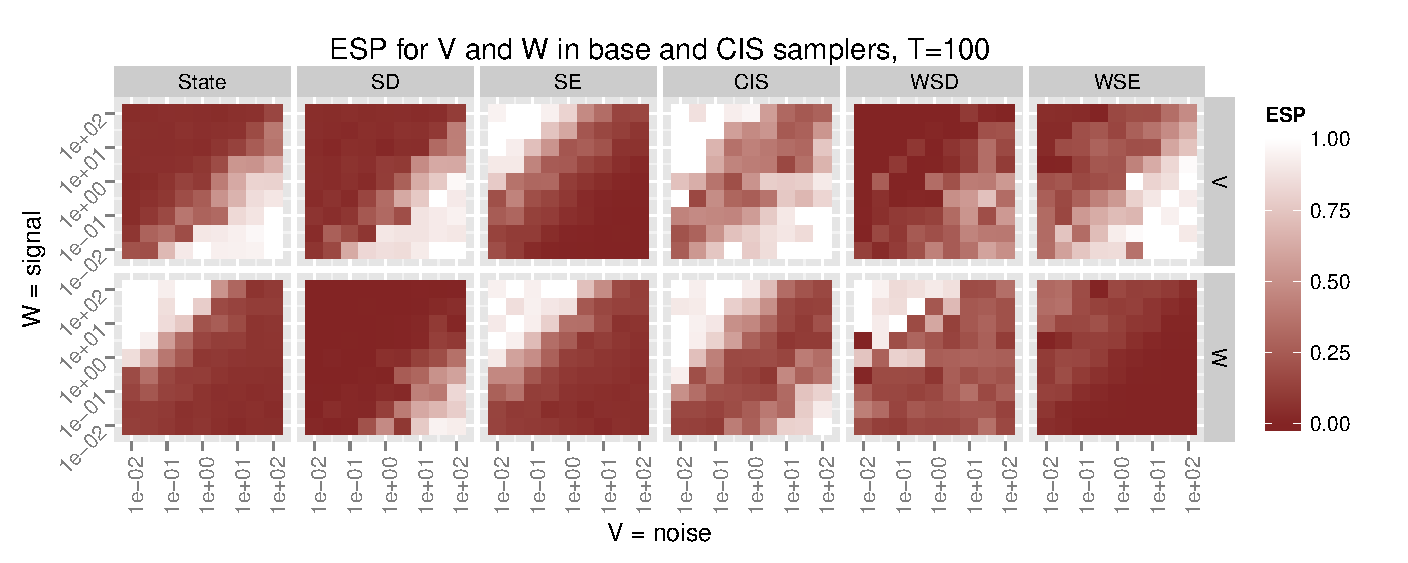
\includegraphics[width=\textwidth]{basecisESplot100}
\caption{}
\label{fig:ESPa}
\end{subfigure}
\begin{subfigure}[b]{0.53\textwidth}
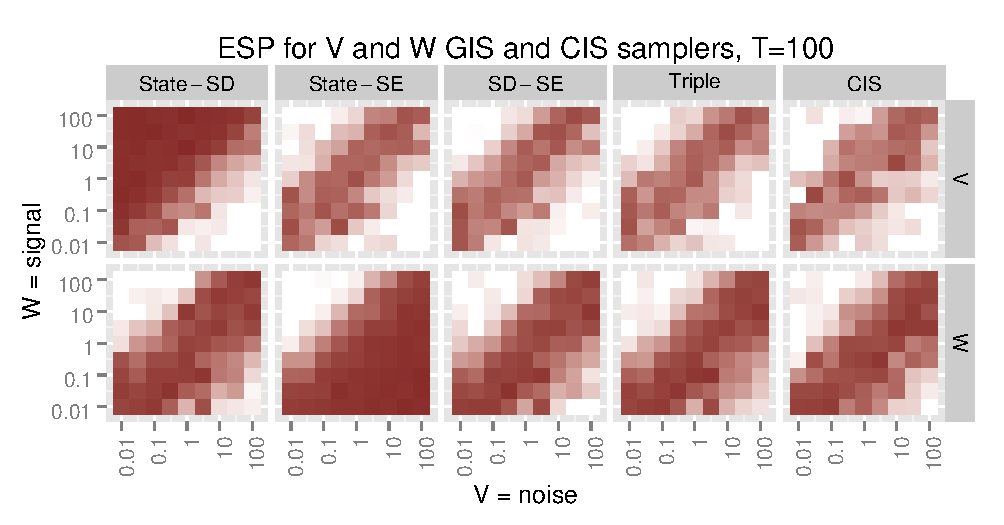
\includegraphics[width=\textwidth]{altintESplotV100}
\caption{}
\label{fig:ESPb}
\end{subfigure}
\begin{subfigure}[b]{0.45\textwidth}
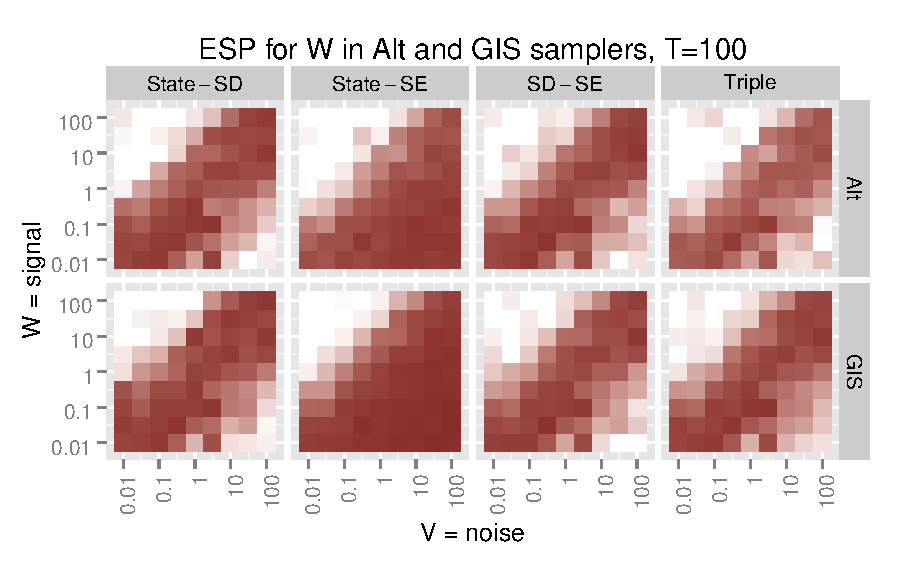
\includegraphics[width=\textwidth]{altintESplotW100}
\caption{}
\label{fig:ESPc}
\end{subfigure}
\caption{Effective sample proportion in the posterior sampler for a time series of length $T=100$, for $V$ and $W$ in the each sampler. Figure \ref{fig:ESPa} contains ESP for $V$ and $W$ for the base samplers, Figure \ref{fig:ESPb} contains ESP in the GIS and CIS samplers, and Figure \ref{fig:ESPc} contains ESP in the Alt samplers. $X$ and $Y$ axes indicate the true values of $V$ and $W$ respectively for the simulated data. Note that the signal-to-noise ratio is constant moving up any diagonal. In the upper left the signal is high, in the lower right the noise is high.}
\label{ESplot}
\end{figure}

\setlength{\tabcolsep}{6pt}
\begin{table}
  \centering
  \begin{tabular}{lccccc}\hline
     & State           & SD                 & SE                  & WSD                 & WSE \\\hline
   V & $R^* < 1$       & $R^* < 1$           & $R^* > 1$           & $R^* < 1$           & $R^* < 1$ \\ 
   W & $R^* > 1$       & $R^* < 1$           & $R^* > 1$           & $R^* > 1$           & $R^* > 1$ \\ \hline
     & State-SD        & State-SE            & SD-SE              & Triple              & CIS \\\hline
   V & $R^* < 1$       & $R^* \not\approx 1$ & $R^* \not\approx 1$ & $R^* \not\approx 1$ & $R^* \not\approx 1$ \\
  W  &$R^* \not\approx 1$& $R^* > 1$          & $R^* \not\approx 1$ & $R^* \not\approx 1$ & $R^* \not\approx 1$\\\hline
  \end{tabular}
  \caption{Rule of thumb for when each sampler has a high ESP for each variable as a function of the true signal-to-noise ratio, $R^*=W^*/V^*$. The bottom panel of the table applies to both the interweaving and alternating algorithms. Note that as the length of the time series increases, the farther away from one $R^*$ has to be for a given sampler to have a high ESP.}
  \label{tab:stnmix}
\end{table}

We fit the LLM to the simulated datasets using several GIS samplers and a CIS sampler as well. Since the wrongly-scaled samplers behaved similarly to the state sampler and neither of the underlying DAs were a SA for $V$ and $W$ jointly, we ignored them in the construction of the GIS samplers. Instead, we constructed the State-SD, State-SE, SD-SE, and Triple (State-SD-SE) GIS samplers, as well as the CIS sampler. Figure \ref{fig:ESPb} has plots of ESP for each of the GIS and CIS algorithms while Figure \ref{fig:ESPc} has plots of ESP for each of the Alt algorithms. Table \ref{tab:stnmix} summarizes the results on the bottom.

Essentially, each GIS and Alt algorithm has high ESP when at least one of the base algorithms has high ESP. For example, the State-SD GIS and Alt algorithms have high ESP for $W$ except for a narrow band where $R^*$ is near one while ESP is high for $W$ in the state sampler when $R^*>1$ and in the SD sampler when $R^*<1$. Similarly in the State-SD GIS and Alt algorithms, mixing for $V$ is identical to the State and SD samplers since neither sampler improves on the other in any region of the parameter space. Both the State-SD GIS and Alt algorithms take advantage of the fact that the state and SD DA algorithms make up a ``beauty and the beast'' pair for $W$ and thus improves mixing in the marginal chain for $W$. However, GIS without an SA-AA pair does not appear to improve on Alt. In Section \ref{sec:Algs:CIS} we noted that the CIS and the SD-SE GIS algorithms consist of the same steps, just rearranged. This suggests that they should perform similarly and in fact the SD-SE GIS algorithm behaves essentially identically to the CIS and Triple GIS algorithms. We also include simulations with differing sizes of $T$ using these samplers in the supplementary materials (Appendix M). Like with the base samplers, increasing the length of the time series worsens ESP for both $V$ and $W$ in all samplers and in particular shrinks the area of the parameter space in which ESP is high.

In Appendix L of the supplementary materials we also compare the time required to adequately characterize the posterior distribution between various algorithms, taking into account both mixing and computational time. GIS and Alt perform essentially identical in this respect, though there is good reason to expect GIS to sometimes be more efficient. In Appendix N we show that for very long time series, GIS does become significantly more efficient than Alt.


\section{Discussion}\label{sec:Discuss}

In order to explore reparameterizing the DA and apply the interweaving strategies of \citet{yu2011center} in dynamic linear models, we start with two DAs, the latent states and the scaled disturbances, and introduce three new DAs for the DLM: the scaled errors, the wrongly-scaled disturbances, and the wrongly-scaled errors. Using these DAs, we construct several alternating algorithms and GIS algorithms and a CIS algorithm. We also find under some assumptions that any SA for a general class of DLMs yields a full conditional distribution for the model parameters that is as difficult to sample from as the target posterior. With the available DAs, we construct each possible DA algorithm, several GIS algorithms and their corresponding Alt algorithms, and a CIS algorithm for the general DLM and test these algorithms in the local level model using a simulation study. We find that the true signal-to-noise ratio, $R^*=V^*/W^*$, is important for determining when each algorithm performs well, and in addition that there appears to be no substantive difference in mixing between a GIS algorithm an its corresponding Alt algorithm. In fact, the three best performing algorithms under most circumstances are the SD-SE GIS algorithm, the SD-SE Alt algorithm and the CIS algorithm. The only caveat is that for very long time series the GIS version of an algorithm will start to become relatively efficient. 

The importance of the true signal-to-noise ratio in DLMs to the mixing and convergence properties of various MCMC algorithms has been anticipated in the literature. In the AR(1) plus noise model, \citet{pitt1999analytic} find that the signal-to-noise ratio along with the AR(1) coefficient determine the convergence rate of a Gibbs sampler. In addition, they find that the convergence rate decreases as the length of the time series increases, which is consistent with our empirical findings in the local level model. When \citet{fruhwirth2004efficient} study the dynamic regression model with a stationary AR(1) process on the regression coefficient, they use both the states and the scaled disturbances (non-centered disturbances) and several other DAs motivated by some results for Gibbs samplers in the hierarchical model literature. When examining the behavior of the resulting DA algorithms, they find that the relative behavior of the SD sampler and the State sampler depends on a function of the true signal-to-noise ratio that also depends on the true value of the autocorrelation parameter and the distribution of the covariate. In addition none of the other DA algorithms they consider are more efficient than both the state sampler and the SD sampler at the same time. Given this previous work, it is likely that in the general DLM the signal-to-noise ratio will in some way determine how well each algorithm performs even if we do not know the precise manner in which it affects mixing and convergence behavior. This is probably consequence of the relevance of the Bayesian fraction of missing information and the related EM fraction of missing information to the performance of the DA and EM algorithms (see \citet{van2001art} for a good explication of both concepts).

A major computational bottleneck in most of our algorithms occurs when we have to draw from $p(W|V,\gamma,y)$, $p(V|W,\psi,y)$, $p(V|W,\tilde{\gamma},y)$ or $p(W|V,\tilde{\psi},y)$. The densities $p(W|V,\gamma,y)$ and $p(V|W,\psi,y)$ have the form
\[
p(x)\propto x^{-\alpha-1}\exp\left[-ax + b\sqrt{x} - c/x\right],
\]
while the densities $p(W|V,\tilde{\psi},y)$ and $p(V|W,\tilde{\gamma},y)$ have the form
\[
p(x)\propto x^{-\alpha-1}\exp\left[ -ax + b/\sqrt{x} -c/x\right]
\]
where $\alpha,a,c>0$ and $b\in\Re$. When $b=0$ we have a special case of the generalized inverse Gaussian (GIG) distribution, so perhaps the methods used to speed up draws from the GIG can be used here \citep{jorgensen1982statistical,dagpunar1989easily,devroye2012random}. On the other hand, it might be worth putting effort into drawing $V$ and $W$ jointly. Using the scaled disturbances, the conditional distribution of $V$ given $W$ is inverse gamma in the LLM and inverse Wishart in the general DLM, so it is easy to derive the marginal density $p(W|\gamma,y)$ up to a proportionality constant. In our LLM example, this density turns out to be very difficult to sample from and in particular, it is not easy to come up with a generally good approximation for rejection sampling or for a Metropolis step. The problem could be solved by a more judicious choice of priors --- we chose inverse Wishart priors for $V$ and $W$ partially because they are standard and partially because their conditional conjugacy with the states is computationally convenient, but outside of the state sampler there may be a more convenient prior. In addition, there are well known inferential problems with the inverse Wishart prior in the hierarchical model literature, e.g. \citet{gelman2006prior}\if0\blind and \citet{alvarez2014cov}\fi, though it is unclear whether this transfers over to DLMs or more generally any time series model. An alternative is to use the conditionally conjugate prior conditional on the scaled disturbances, or whichever DA we prefer. In the LLM, the conditionally conjugate prior for $\sqrt{W}$ using the scaled disturbances as the DA is a Gaussian distribution --- strictly speaking this prior is on $\pm \sqrt{W}$. If we use this prior for $\pm\sqrt{V}$ as well, the $V$ step in the scaled disturbance sampler becomes a draw from the generalized inverse Gaussian distribution. This prior has been used by \citet{fruhwirth2011bayesian} and \citet{fruhwirth2008bayesian} to speed up computation while using the scaled disturbances in hierarchical models and by \citet{fruhwirth2010stochastic} for time series models with a DA similar to the scaled disturbances. We omit the results here, but using this prior on both variances does not alter our mixing results for any of the MCMC samplers. There is a trade-off in computation time to consider --- for example when using the scaled disturbances, the draw of $W|V,\gamma,y$ is sped up by using the Gaussian prior on $\pm\sqrt{W}$ since it becomes a Gaussian draw while the $V|W,\gamma,y$ is slower since it becomes a generalized inverse Gaussian draw instead of an inverse gamma. The gains outweigh the costs, at least in the local level model. 

In the general DLM, however, it is unclear whether this will hold because of the additional complications stemming from $V$ and $W$ being matrices. The conditionally conjugate prior for $W$ given $\gamma$ is a normal distribution on $\pm L_W$, or in the case of $V$ given $\psi$, a normal distribution on $\pm$ $L_V$. But the full conditional for the other covariance matrix becomes a matrix analogue of the generalized inverse Gaussian distribution, which appears difficult to sample from. So no matter which conditionally conjugate prior is used under the scaled errors or scaled disturbances, one of $V$ or $W$'s full conditionals will be intractable. This is not a problem for the DA algorithms necessarily -- you have the freedom to use the inverse Wishart prior for $V$ and the normal prior for $\pm L_W$ in the scaled disturbance sampler, for example. But in any interweaving or alternating algorithm each covariance matrix needs to be drawn from two full conditionals -- one given each of the DAs used in the algorithm, yielding at least one intractable full conditional. A Metropolis step is probably a tolerable solution to the problem, though the details of how to best accomplish this will likely have to be determined on a case by case basis.

\section{Supplementary materials}\label{sec:Supp}
All supplementary materials are available in a single \verb0.zip0 file.
\begin{description}
\item[appendices.pdf:] This file provides 8 appendices cited in the main article:
\begin{itemize}
\item[] Appendix A: Derivation of marginal model for the DLM.
\item[] Appendix B: Proof of lemma 1.
\item[] Appendix C: Construction of the wrongly-scaled DA algorithms.
\item[] Appendix D: Derivations of joint and full conditional distributions for each DA in the DLM.
\item[] Appendix E: MCFA for simulation smoothing.
\item[] Appendix F: Further augmentation for non-invertible $F_t$.
\item[] Appendix G: Efficiently drawing from $p(W|V,\gamma,y)$ and $p(V|W,\psi,y)$ in the LLM.
\item[] Appendix H: Efficiently drawing from $p(W|V,\tilde{\gamma},y)$ and $p(V|W,\tilde{\psi},y)$ in the LLM.
\item[] Appendix I: Equivalence of CIS and SD-SE GIS in the DLM.
\item[] Appendix J: Partial CIS Algorithms in the DLM.
\item[] Appendix K: Using posterior correlations to understand patterns of ESP.
\item[] Appendix L: Computational time for each algorithm.
\item[] Appendix M: Additional plots for other values of $T$.
\item[] Appendix N: Comparing GIS and Alt in very long time series.
\end{itemize}

\item[mcfa.R:] This file contains R code to perform the MCFA for obtaining a draw from $p(\theta|V,W,y)$ and from $p(\psi|V,W,y)$ in the local level model.

\item[dlmasisfun.R:] This file contains many R functions for obtaining the simulations from a variety of MCMC algorithms in the local level model, summarizing those simulations appropriately, and for simulating data from the model. It depends on \verb0wscalerej.R0.

\item[wscalerej.R] This file contains several R functions for obtaining simulations from the wrongly-scaled DA algorithms in the local level model.

\item[dlmasismixrun.R:] This file contains R code that uses the functions in \verb0dlmasisfun.R0 and \verb0mcfa.R0 to obtain the simulations used in the local level model example from Section \ref{sec:LLM}.

\item[dlmasislongfun.R:] This file contains a modified version of the R functions in \verb0dlmasisfun.R0 in order to accomodate simulations for very long time series.

\item[dlmasislongrun.R:] This file contains R code that uses the functions in \verb0dlmasislongfun.R0 to obtain simulations for long time series in the local level model used in Appendix L.

\item[plots.R:] This file contains R code that uses the output from \verb0dlmasismixrun.R0 to create the various plots in the main document and the appendices.

\end{description}


\clearpage
\bibliographystyle{MWS_jasa}  % proper bibliography style for ASA
\bibliography{dlmasis}
\end{document}
